\section{Experimental Results and Empirical Evaluation}
\label{sec:results}

We report final test performance averaged across three independent random seeds (0, 1, 2) on the frozen test partitions. In alignment with regulatory screening requirements where toxic hits are heavily outnumbered by non-toxic chemicals, Precision-Recall AUC (PR~AUC) serves as our primary decision metric, complemented by ROC~AUC.

\begin{table}[htbp]
\centering
\caption{Overall Performance on Held-Out Test Partitions (Mean $\pm$ Sample Standard Deviation across 3 Seeds)}
\label{tab:main_results}
\begin{tabular}{llcccc}
\toprule
\textbf{Model} & \textbf{Modality / Input} & \multicolumn{2}{c}{\textbf{Scaffold Test}} & \multicolumn{2}{c}{\textbf{Random Test}} \\
\cmidrule(lr){3-4} \cmidrule(lr){5-6}
& & \textbf{PR AUC} & \textbf{ROC AUC} & \textbf{PR AUC} & \textbf{ROC AUC} \\
\midrule
\multicolumn{6}{l}{\textit{Phase 1 Classical Baselines (Frozen)}} \\
RF & Morgan+Desc & $0.4035 \pm 0.0042$ & $0.7762 \pm 0.0020$ & $0.5456 \pm 0.0038$ & $0.8607 \pm 0.0045$ \\
XGBoost & Morgan+Desc & $0.4010 \pm 0.0045$ & $0.7606 \pm 0.0036$ & $0.5647 \pm 0.0021$ & $0.8621 \pm 0.0019$ \\
RF & Morgan & $0.3703 \pm 0.0016$ & $0.7288 \pm 0.0063$ & $0.5038 \pm 0.0006$ & $0.8364 \pm 0.0039$ \\
XGBoost & Morgan & $0.3180 \pm 0.0020$ & $0.7020 \pm 0.0025$ & $0.5046 \pm 0.0017$ & $0.8072 \pm 0.0013$ \\
LogReg & Morgan+Desc & $0.3122 \pm 0.0000$ & $0.7317 \pm 0.0000$ & $0.4818 \pm 0.0000$ & $0.8405 \pm 0.0000$ \\
LogReg & Morgan & $0.3116 \pm 0.0000$ & $0.7156 \pm 0.0000$ & $0.4821 \pm 0.0000$ & $0.8212 \pm 0.0000$ \\
\midrule
\multicolumn{6}{l}{\textit{Phase 2 Deep Learning and Hybrid Models}} \\
\textbf{H2: Ensemble} & XGB + H1 & $\mathbf{0.3945 \pm 0.0011}$ & $\mathbf{0.7643 \pm 0.0017}$ & $\mathbf{0.5626 \pm 0.0034}$ & $\mathbf{0.8604 \pm 0.0036}$ \\
\textbf{H1: Hybrid} & MPNN + Desc & $0.3553 \pm 0.0057$ & $0.7384 \pm 0.0067$ & $0.5153 \pm 0.0107$ & $0.8374 \pm 0.0048$ \\
FP-MLP & Morgan + Desc & $0.3429 \pm 0.0106$ & $0.7269 \pm 0.0054$ & $0.5378 \pm 0.0090$ & $0.8507 \pm 0.0061$ \\
\bottomrule
\end{tabular}
\end{table}

\begin{figure}[htbp]
\centering
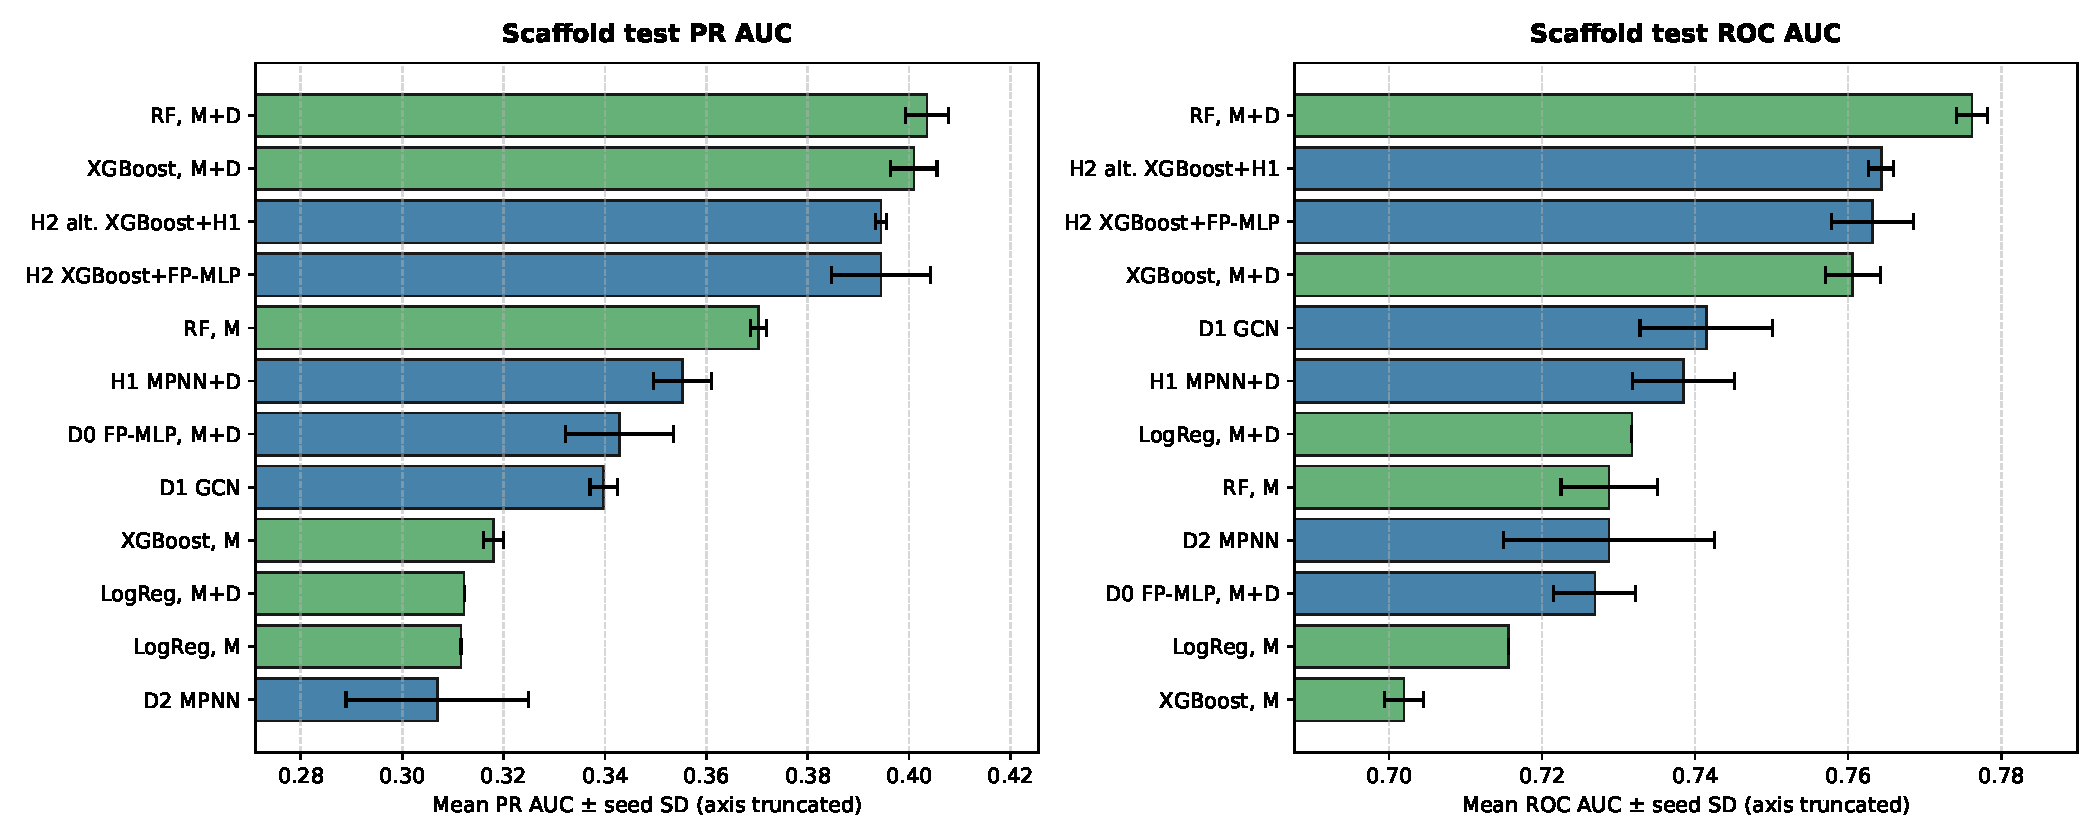
\includegraphics[width=0.48\textwidth]{figures/mean_pr_roc_scaffold.pdf}
\caption{Mean PR~AUC and ROC~AUC performance on the Bemis--Murcko scaffold test set across model architectures. Deep learning models are highlighted in blue; classical tree baselines in green.}
\label{fig:mean_scaffold}
\end{figure}

\subsection{Benchmark Performance on Bemis--Murcko Scaffolds}
Table~\ref{tab:main_results} and Figure~\ref{fig:mean_scaffold} summarize test performance under the primary scaffold partitioning regime:
\begin{itemize}
    \item \textbf{Graph Representation vs. Flat Neural Control:} The H1 hybrid (\texttt{mpnn+desc}) attains a mean scaffold PR~AUC of $0.3553 \pm 0.0057$ and ROC~AUC of $0.7384 \pm 0.0067$. It consistently outperforms the FP-MLP control (\texttt{fpmlp+both}, PR~AUC $0.3429 \pm 0.0106$) by $+0.0124$ PR~AUC. Because both models utilize the identical 213 RDKit descriptors, this gain isolates the structural representation advantage of learned continuous message passing over discrete 2,048-bit Morgan fingerprints.
    \item \textbf{Synergy via Late-Fusion Ensembling (H2):} The H2 ensemble (\texttt{ens\_xgb\_mpnn+desc}) achieves PR~AUC $0.3945 \pm 0.0011$ and ROC~AUC $0.7643 \pm 0.0017$. H2 establishes the lowest seed standard deviation ($\sigma_{\text{PR}} = 0.0011$) among all evaluated architectures, delivering a highly stable predictive system.
    \item \textbf{Classical Tree Baselines on Handcrafted Descriptors:} Random Forest ($0.4035$) and XGBoost ($0.4010$) trained on concatenated Morgan fingerprints and physicochemical descriptors remain the top-performing individual models on this dataset, consistent with findings by Jiang et al.~\cite{jiang2021could}.
\end{itemize}

\begin{figure}[htbp]
\centering
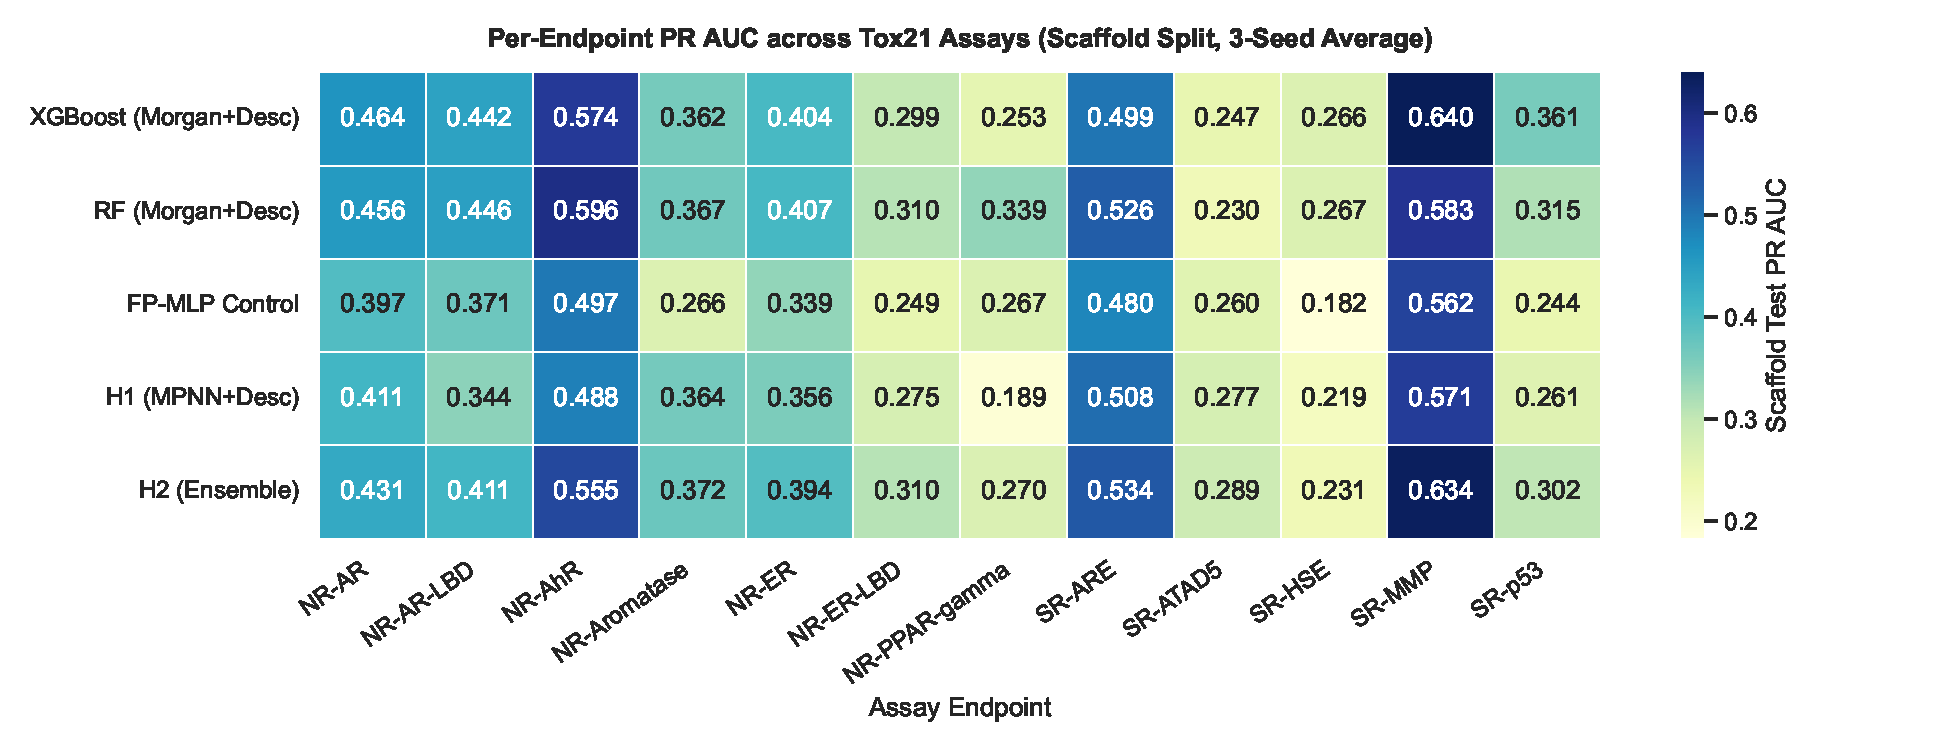
\includegraphics[width=0.48\textwidth]{figures/per_endpoint_heatmap_comparison.pdf}
\caption{Per-endpoint PR~AUC heatmap across all 12 Tox21 assays on the scaffold test partition (averaged across 3 seeds).}
\label{fig:heatmap}
\end{figure}

\subsection{Per-Endpoint Performance and Assay Heterogeneity}
Figure~\ref{fig:heatmap} breaks down PR~AUC across all 12 individual assay endpoints. Performance exhibits substantial biological heterogeneity across pathways:
\begin{itemize}
    \item On highly responsive nuclear receptor assays such as \texttt{NR-AhR} and \texttt{NR-AR}, models achieve robust PR~AUC values between $0.45$ and $0.62$.
    \item Conversely, on sparse, difficult stress response assays such as \texttt{SR-HSE} and \texttt{SR-MMP}, precision drops across all models.
    \item The H1 hybrid achieves substantial gains over the FP-MLP control on endpoints such as \texttt{NR-Aromatase} ($+0.1274$), \texttt{SR-HSE} ($+0.0507$), and \texttt{SR-ARE} ($+0.0455$).
\end{itemize}

\subsection{Statistical Hypothesis Testing and Bootstrap Analysis}
Because Tox21 provides only 12 assay endpoints, paired Wilcoxon signed-rank tests are reported alongside endpoint win/loss counts and joint non-parametric bootstrap confidence intervals:
\begin{enumerate}
    \item \textbf{H1 vs.\ FP-MLP:} H1 wins on \textbf{9 of the 12 endpoints} (mean difference $+0.0124$, $p = 0.1514$). While the Wilcoxon test has modest power at $N=12$, the $9/3$ win ratio demonstrates consistent representational superiority.
    \item \textbf{H2 Ensemble vs.\ H1 Hybrid:} H2 wins on \textbf{12 of 12 endpoints} (mean difference $+0.0392$, $p = 0.00049$), providing conclusive statistical proof of ensemble complementarity.
    \item \textbf{H2 Ensemble vs.\ XGBoost:} H2 and XGBoost perform comparably across endpoints (5 wins, 7 losses, mean difference $-0.0065$, $p = 0.6221$), while H2 reduces prediction variance by more than $4\times$ over XGBoost ($\sigma = 0.0011$ vs.\ $0.0045$).
\end{enumerate}

Joint paired percentile bootstrap sampling (1,000 resamples on test predictions) further confirms these findings: on \texttt{NR-Aromatase}, H1 achieves a statistically significant 95\% CI gain over FP-MLP of $[+0.035, +0.224]$. Across 10 of 12 assays, the 95\% CI for H2 over H1 strictly excludes zero on the positive side.

\begin{figure}[htbp]
\centering
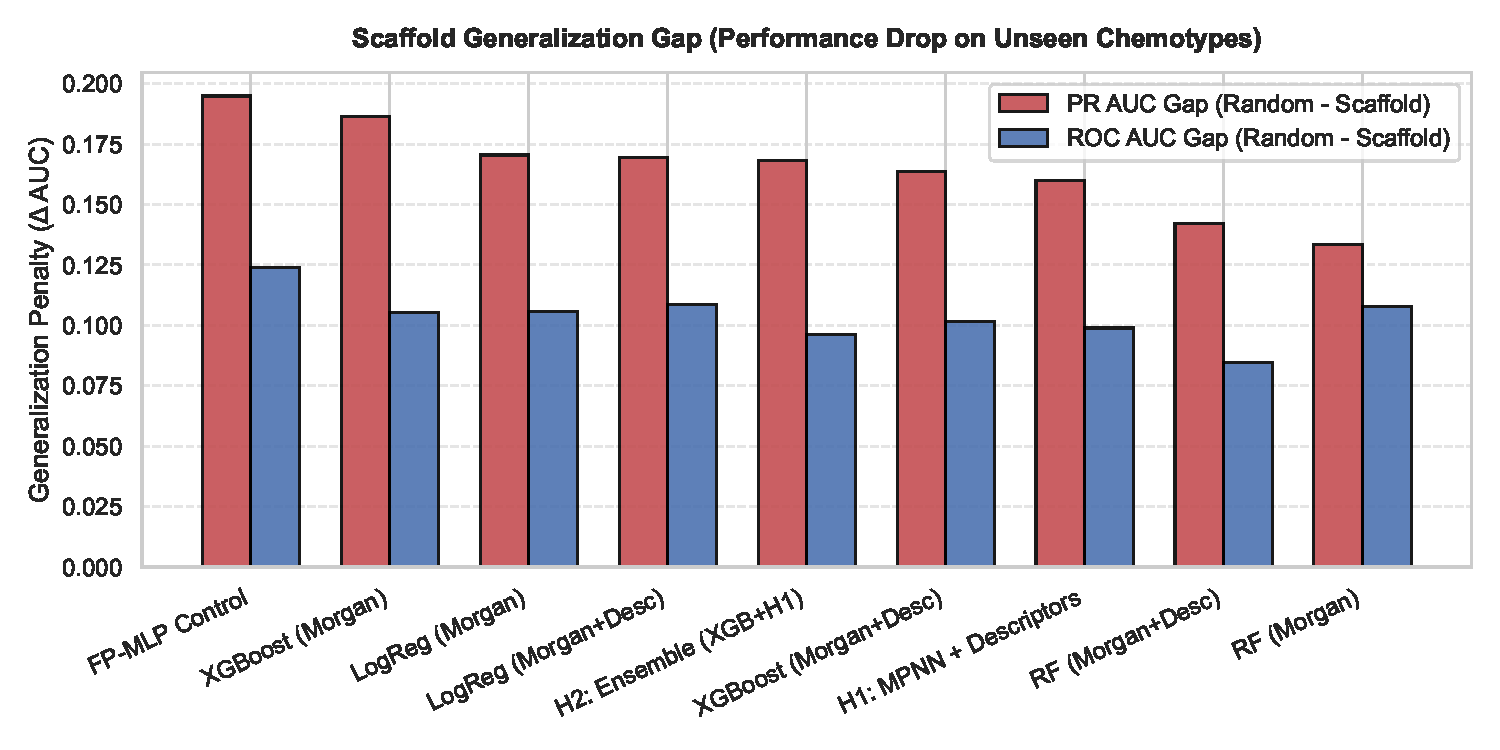
\includegraphics[width=0.48\textwidth]{figures/generalization_gap.pdf}
\caption{Chemical generalization penalty ($\Delta \text{AUC} = \text{Random} - \text{Scaffold}$) quantifying performance degradation on unseen molecular frameworks.}
\label{fig:gap}
\end{figure}

\subsection{Chemical Generalization Gap}
Figure~\ref{fig:gap} plots the performance drop observed when transitioning from random to scaffold evaluation. Every model experiences a large generalization penalty ($\Delta\text{PR} \approx 0.160$--$0.195$ and $\Delta\text{ROC} \approx 0.085$--$0.124$). 

Notably, the FP-MLP exhibits the largest PR~AUC generalization drop ($\Delta\text{PR} = 0.1949$), reflecting the tendency of dense networks to overfit fixed fingerprint bit patterns. In contrast, the H1 graph hybrid demonstrates superior scaffold robustness ($\Delta\text{PR} = 0.1600$), confirming that learned message passing features transfer better across scaffold shifts than memorized fingerprint fragments.

\begin{table}[htbp]
\centering
\caption{Ablation Suite on H1 Architecture (Scaffold Split, 3 Seeds)}
\label{tab:ablations}
\begin{tabular}{llcc}
\toprule
\textbf{Configuration} & \textbf{Description / Modification} & \textbf{PR AUC} & \textbf{ROC AUC} \\
\midrule
\textbf{Reference H1} & MPNN + 2D RDKit Descriptors & $\mathbf{0.3553}$ & $\mathbf{0.7384}$ \\
Ablation A6c & MPNN + Morgan + Descriptors (\texttt{both}) & $0.3309$ & $0.7186$ \\
Ablation A6b & MPNN + Morgan Fingerprints (\texttt{morgan}) & $0.2614$ & $0.6699$ \\
\textbf{Ablation A6a} & \textbf{Shuffled Descriptors (Negative Control)} & $\mathbf{0.2547}$ & $\mathbf{0.6951}$ \\
\bottomrule
\end{tabular}
\end{table}

\begin{figure}[htbp]
\centering
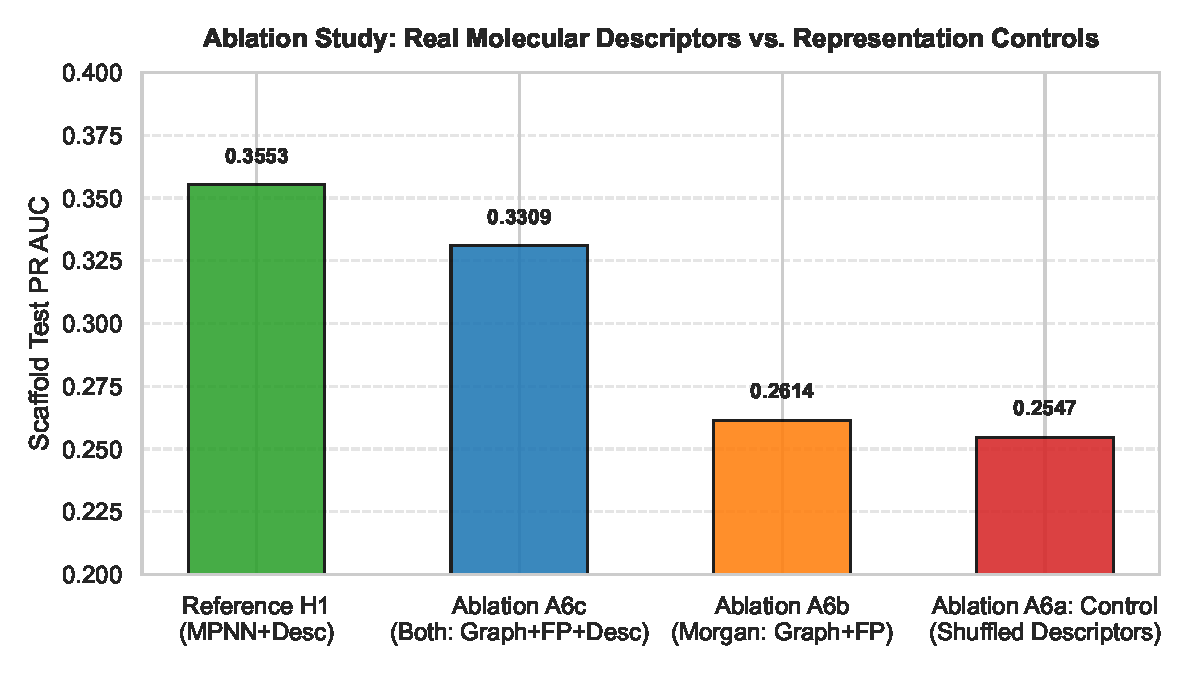
\includegraphics[width=0.45\textwidth]{figures/ablation_study.pdf}
\caption{Impact of input representations and negative controls on scaffold test PR~AUC.}
\label{fig:ablation_fig}
\end{figure}

\subsection{Ablation Suite and Negative Control Verification}
Table~\ref{tab:ablations} and Figure~\ref{fig:ablation_fig} detail the results of the ablation suite:
\begin{itemize}
    \item \textbf{Shuffled-Descriptor Control (\texttt{shuffled\_desc}):} When descriptor rows are permuted across molecules, performance crashes from $0.3553$ to $0.2547$ ($-0.1006$ PR~AUC; a $28.3\%$ collapse). This decisively refutes the hypothesis that hybrid gains are caused by parameter capacity or unspecific regularization.
    \item \textbf{Representation Substitution (\texttt{morgan}):} Replacing continuous descriptors with sparse 2,048-bit Morgan fingerprints drops PR~AUC to $0.2614$, proving that high-dimensional sparse vectors introduce severe optimization interference in deep graph architectures.
\end{itemize}

\begin{figure}[htbp]
\centering
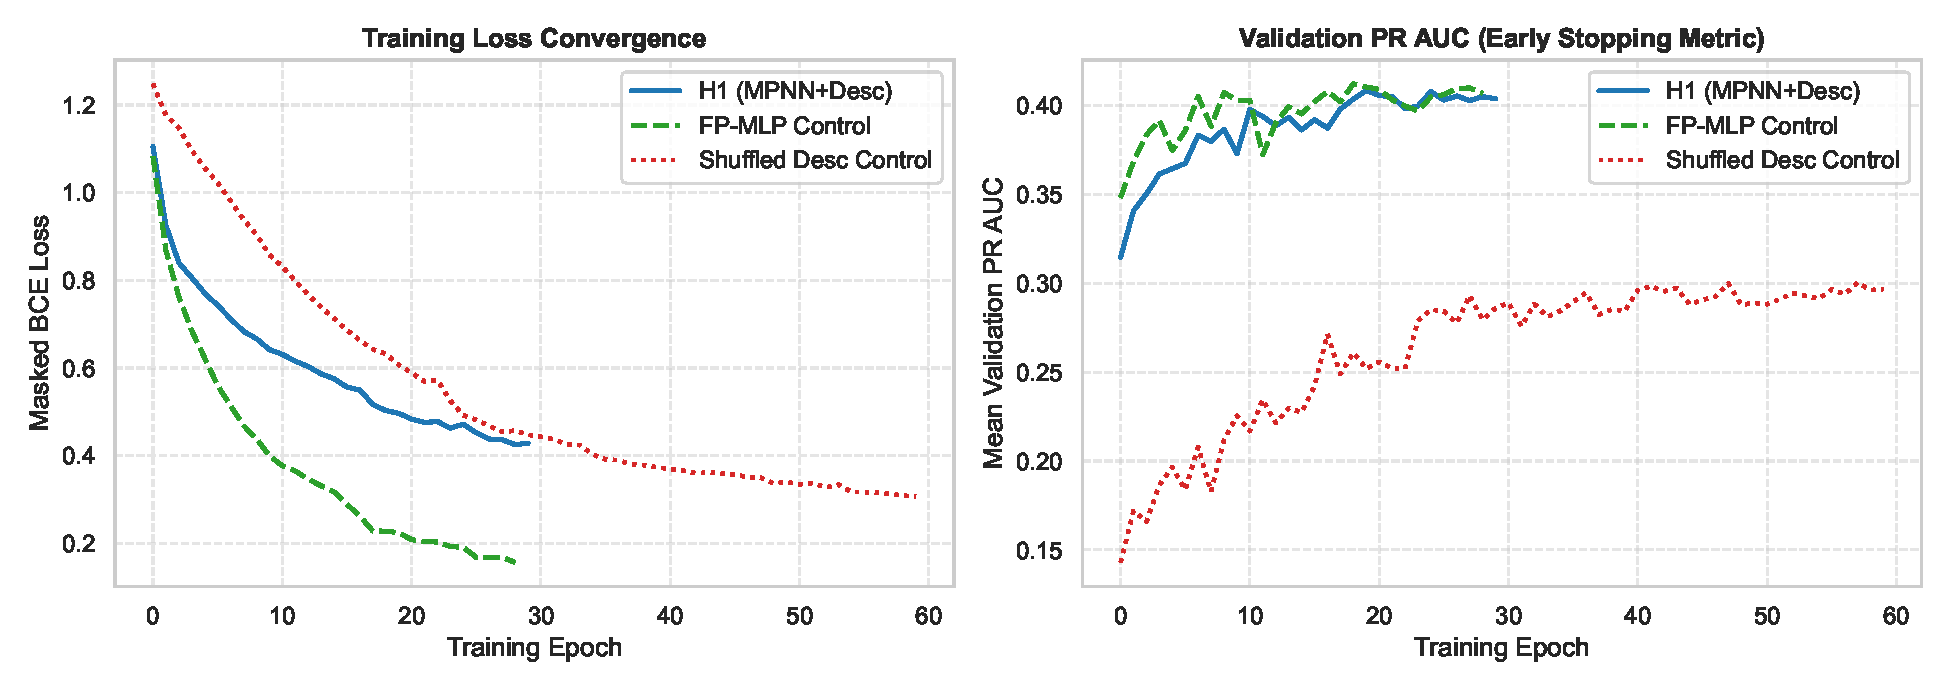
\includegraphics[width=0.48\textwidth]{figures/dl_learning_curves.pdf}
\caption{Training loss convergence and validation PR~AUC trajectory across training epochs.}
\label{fig:curves}
\end{figure}

\subsection{Optimization Dynamics and Learning Curves}
Figure~\ref{fig:curves} illustrates the training trajectories. Masked BCE loss decreases smoothly for H1, reaching optimal validation PR~AUC at epoch 19 ($0.4085$) before triggering early stopping restoration. The shuffled-descriptor control exhibits slower loss descent and lower plateau validation PR~AUC, confirming impaired learning dynamics.
